\pdfoutput=1
\documentclass[10pt]{beamer}

%STANDARD PREAMBLE
%https://tex.stackexchange.com/questions/68821/is-it-possible-to-create-a-latex-preamble-header
\usepackage{../../rsrc/beamer_preamble}

% EMBED ANIMATIONS
% Reference: https://tex.stackexchange.com/questions/240243/getting-gif-and-or-moving-images-into-a-latex-presentation
%\usepackage{xmpmulti}
\usepackage{animate}

%%% SPECIFIC TO THIS DOC
\newcommand{\obs}{x^{(i)} }
\newcommand{\alatent}{z^{(i)} }
\newcommand{\N}{\mathcal{N}}
\newcommand{\I}{\mathbb{I}}
%%% SKIP TO BOTTOM OF SLIDE
%https://tex.stackexchange.com/questions/54180/how-do-i-write-something-at-the-end-of-the-slide-in-beamer
\newcommand{\bottom}{\vskip0pt plus 1filll}


\title{Variational Autoencoders}

\begin{document}

\maketitle

\begin{frame}{Table of contents}
  \setbeamertemplate{section in toc}[sections numbered]
  \tableofcontents[hideallsubsections]
\end{frame}

\section{Overview}

\begin{frame}{Overview}
TODO
\end{frame}



%%%%%%%%%%%%%%%%%%%%%%%%%%%%%%%%%%%%%%%%%%%
%%%%%%%%%%%%%%%%%%%%%%%%%%%%%%%%%%%%%%%%%%%
\section{Probabilistic model}

\begin{frame}{Prefatory Notes}
\begin{sblock}{Simplification}
For ease of illustration, we restrict our attention to a variational autoencoder that applies i.i.d assumptions and Gaussian distributions (and therefore real-valued observations) throughout.    Note that neither assumption is necessary. 
\end{sblock}
\end{frame}


\begin{frame}{Probabilistic decoder}
\footnotesize
Consider a parametric frequentist latent variable model, with 
\begin{itemize}
\item observations $x = (\obs)_{i=1}^N, \quad \obs \in \R^d$
\item latent variables $z =(\alatent)_{i=1}^N, \quad \alatent \in \R^k$
\item parameter $\theta$ (fixed but to be learned)
\end{itemize}

Let us model our observations $x$ via the factorization
\[ p_\theta(x |z )= \ds\prod_i \; p_\theta( \obs | \alatent ) \] 
Let the likelihood of each observation $\obs$ be obtained by using a Multi-Layer Perceptron (MLP), parameterized by weights $\theta$, to map latent variable $\alatent$ to Gaussian parameters governing the distribution of observation $x^{(i)}$.
\begin{equation} x^{(i)} | \alatent, \theta \sim \N \big(\mu_{x^{(i)}}( \alatent; \theta), \; \Sigma_{x^{(i)}} (\alatent; \theta) \big)  
\label{likelihood} 
\end{equation}
Since the MLP maps latent variables, $z$, to the parameters of a probability distribution over observed data, $x$, we refer to it as a \bf{probabilistic decoder.}

\vfill

\tiny  Notes on notation
\begin{enumerate}
\item $\N(M,V)$ refers to the Gaussian density with mean $M$ and covariance $V$.
\item $\mu_{\obs}(\alatent; \theta)$ is meant to denote the mean parameter for a distribution over observed datum $\obs$; that parameter is a function of latent variable $z$ and learnable parameter $\theta$. Notation should be similarly interpreted throughout this section.
\end{enumerate}

\end{frame}


\begin{frame}{Probabilistic encoder}
Let us additionally put a prior distribution on the latent variables:
\begin{align*}
p_\theta(z) &= \ds\prod_i  p_\theta(\alatent) = \ds\prod_i  \N(\+0, \I) 
\end{align*}

%And let us assume, as in the context of a frequentist latent variable model, that $\theta$ is a fixed (but unknown) constant that will be learned.  

In this case, the posterior distribution, $p_
\theta(z| x)$, is intractable.  However, we consider an approximation 
by using a Multi-Layer Perceptron (MLP), parameterized by weights $\phi$, to map observation $x$ to Gaussian parameters governing the distribution of latent variable $z$: 
\begin{align}
 q_\phi(z| x) &=  \ds\prod_i \; q_\phi(\alatent| x^{(i)}) \nonumber \\
\alatent| x^{(i)}, \phi &\sim \N \big(\mu_{\alatent} (x^{(i)}; \phi), \Sigma_{\alatent} (x^{(i)}; \phi) \big) \label{approx_posterior} 
\end{align}
 Since the MLP maps observations, $x$, to to the parameters of a probability distribution over latent variables, $z$, we refer to it as a \bf{probabilistic encoder.} 
 
\end{frame}

\begin{frame}{Probabilistic encoder} 

\begin{itemize}
\item  We may regard the probabilistic encoder as an approximation to the posterior distribution over latent variables which
results from using the probabilistic decoder as a likelihood.
\item The probabilistic encoder is sometimes also referred to as a \bf{recognition model}.
\end{itemize}

\end{frame}

\section{Sample Implementation}

\begin{frame}{Sample Implementation}
Following Appendix C.2 of the VAE paper, we provide a sample implementation for the probabilistic encoder and decoder. 
\end{frame}

\begin{frame}{Probabilistic encoding}
\footnotesize
We may, for example, specifically assume that an observation $\obs$ can be probabilistically encoded into latent variable $\alatent$ via the following process

\begin{minipage}{.6\textwidth}
\begin{align*}
h^{(i)} &= \texttt{tanh} (W_1 x^{(i)} + b_1) \\
\mu_{\alatent}&= W_{21} h^{(i)} + b_{21}, \quad \log \sigma^2_{\alatent} = W_{22}h^{(i)}+b_{22} \\
\alatent & \sim \N(\mu_{\alatent}, \Sigma_{\alatent}), \quad \text{where} \; \text{diag}(\Sigma_{\alatent}) = \sigma_{\alatent}^2
\end{align*}
\end{minipage}
\hfill
\begin{minipage}{.3\textwidth}
\begin{center}
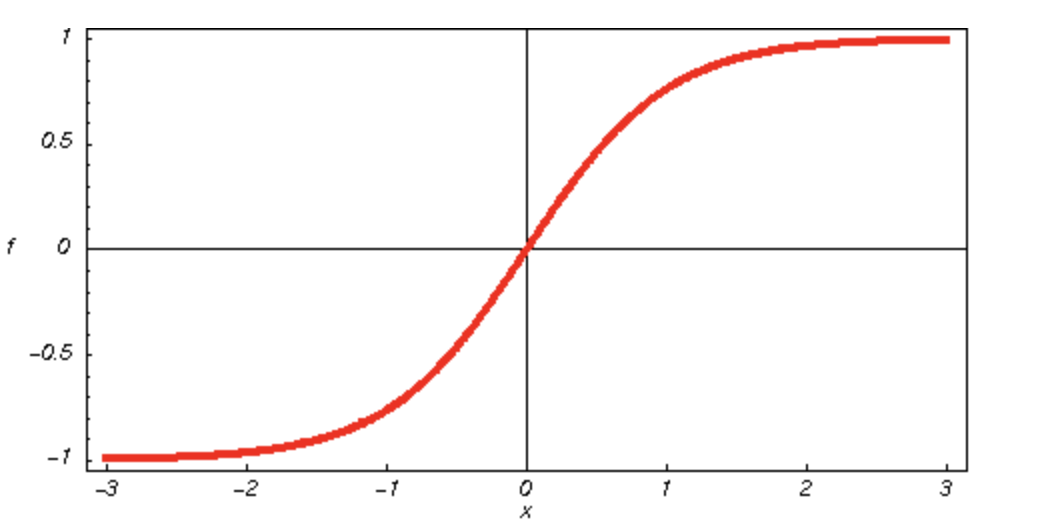
\includegraphics[width=.6\textwidth]{images/tanh}

The hyperbolic tangent (\texttt{tanh}) function
\end{center}
\end{minipage}

where $(W_1, W_{21}, W_{22})$ are the weights and $(b_1, b_{21}, b_{22})$ are the biases of a Multi-Layer Perceptron (MLP). \\
\vfill
Letting $\phi := (W_1, W_{21}, W_{22}, b_1, b_{21}, b_{22})$, we may use the trained encoder to define the approximate posterior, $q_\phi(z| x)$, as defined in \eqref{approx_posterior}.
\end{frame}

\begin{frame}{Probabilistic decoding}
We may, for example, specifically assume that a latent variable $\alatent$ can be probabilistically decoded into  observation $\obs$ via the following process

\begin{align*}
h^{(i)} &= \texttt{tanh} (W_3 \, \alatent + b_3) \\
\mu_{\obs}&= W_{41} h^{(i)} + b_{41}, \quad \log \sigma^2_{\obs} = W_{42}h^{(i)}+b_{42} \\
x|z &\sim \N(\mu_{\obs}, \Sigma_{\obs}), \quad \text{where} \; \text{diag}(\Sigma_{\obs}) = \sigma_{\obs}^2
\end{align*}

where $(W_3, W_{41}, W_{42})$ are the weights and $(b_3, b_{41}, b_{42})$ are the biases of a Multi-Layer Perceptron (MLP). \\
\vfill
 Letting $\theta := (W_3, W_{41}, W_{42}, b_3, b_{41}, b_{42})$, we may use the trained decoder to define the likelihood, $p_\theta(x |z )$, as defined in \eqref{likelihood}.

\end{frame}




\section{Inference}

\begin{frame}{}
We use variational inference to jointly optimize $(\theta, \phi)$.  For example, in our sample implementation, we have 
\begin{align*}
\theta &= (W_3, W_{41}, W_{42}, b_3, b_{41}, b_{42})  && \small \text{generative parameters} \\ 
\phi &= (W_1, W_{21}, W_{22}, b_1, b_{21}, b_{22}) && \small \text{variational parameters}
\end{align*}

In particular, we construct $\mathcal{F}(\theta, \phi; x)$, a lower-bound on the marginal likelihood, $p_\theta(x)$, via the entropy/energy decomposition which is standard in variational inference:   

\begin{equation}
\label{vae_vlbo}
\mathcal{F}(\theta, \phi; x) = \E_{q_\phi(z| x)} [- \log q_\phi(z| x)) + \log p_\theta(x, z ) ]
\end{equation} 
\end{frame}

\begin{frame}{}

We train the model by performing stochastic gradient descent on the variational lower bound $\mathcal{F}$.  During training, the objective function \eqref{vae_vlbo} is approximated by performing a Monte Carlo approximation of the expectation.   Given minibatch $x^{(i)}$, we would like to take $L$ samples from $q_\phi(z| x^{(i)})$ and obtain the following estimator:

\begin{equation}
\label{vae_sgvb}
 \mathcal{F}(\theta, \phi; x^{(i)}) \approx \df{1}{L} \ds\sum_{l=1}^L - \log q_\phi(z^{(i,l)} | x^{(i)}) + \log p_\theta( x^{(i)}, z^{(i,l)} ) 
\end{equation} 
\end{frame}

\begin{frame}{}
However, naively backpropagating gradients in this case would ignore the role of the parameter in the sampling step. Thus, we use the \bf{reparameterization trick} ; i.e. we construct a differentiatiable transformation $g_\phi$ of parameterless distribution $p(\epsilon)$ such that $g_\phi(\epsilon, \obs)$ has the same distribution as $q_\phi(\alatent| x^{(i)})$.\footnote{In this case, since our variational distribution is a multivariate normal, $p(\epsilon)$ is simply a Gaussian with zero mean and identity covariance.}  Using this trick, we take $L$ samples $\{\epsilon_1, ..., \epsilon_L \}$ from $p(\epsilon)$ and obtain the estimator: 

\begin{equation}
\label{vae_sgvb}
 \mathcal{F}(\theta, \phi; x^{(i)}) \approx \df{1}{L} \ds\sum_{l=1}^L - \log q_\phi \big(g_\phi(\epsilon^{(l)}, x^{(i)}) | x^{(i)} \big) + \log p_\theta \big( x^{(i)}, g_\phi(\epsilon^{(l)}, x^{(i)}) \big) 
\end{equation} 

\end{frame}

\section{Anomaly Scoring}

\begin{frame}{Anomaly Scoring}
A straightforward approach to assessing anomalousness of sample $x^{(i)}$ using a Variational Autoencoder was provided by the authors below.   First, take $L$ samples, $\{z^{(i,1)}, ..., z^{(i,L)} \}$ from the fitted variational distribution (i.e, the encoder), $q_\phi(\alatent| x^{(i)})$ .   Each such sample, $z^{(i,l)}$, determines a specific form of the fitted likelihood (i.e. the decoder) by specifying its parameters, $p_\theta(\obs | z^{(i,l)}) = p_\theta(\obs | \mu_{\obs} (z^{(i,l)}), \Sigma_{\obs} (z^{(i,l)})) $. Using this, the \textit{reconstruction probability} of the sample can be defined as the mean of these likelihoods:

\[ \texttt{reconstruction probability}(x^{(i)}) := \df{1}{L} \ds\sum_{l=1}^L p_\theta \big(\obs \cond \mu_{\obs} (z^{(i,l)}) \, , \, \Sigma_{\obs} (z^{(i,l)}) \big)\]
\vfill \vfill
\hfill \tiny An, J., \& Cho, S. (2015). Variational autoencoder based anomaly detection using reconstruction probability. Special Lecture on IE, 2(1).
\end{frame}

\end{document}


    

    



%%%%%%%%%%%%%%%%%%%%%%%%%%%%%%%%%%%%%%%%%%%
%%%%%%%%%%%%%%%%%%%%%%%%%%%%%%%%%%%%%%%%%%%








%%%%%%%%%%%%%%%%%%%%%%%%%%%%%%%%%%%%%%%%%%%%
%\subsubsection{Some Implementational Details}
%
%\begin{itemize}
%\item Note that StrangeNet uses \texttt{pytorch}'s default initialization for the weights and biases of a linear layer, namely a random draw from $\mathcal{U} \big( [-\sqrt{k}, \sqrt{k}] \big)$, where $k=1/\text{\# of input features}$.  This is called a \textit{xavier initialization}. 
%\end{itemize}

%%%%%%%%%%%%%%%%%%%%%%%%%%%%%%%%%%%%%%%%%%%
%%%%%%%%%%%%%%%%%%%%%%%%%%%%%%%%%%%%%%%%%%%
\subsection{Anomaly Scoring}



\end{document}